\documentclass[12pt]{article}
\usepackage{fontspec}
\usepackage{polyglossia}

\setmainlanguage{greek}
\setotherlanguages{english}
\setmainfont{FreeSerif}

\usepackage{graphicx} % Για εισαγωγή εικόνων
\usepackage{geometry} % Για τη διάταξη της σελίδας
\usepackage{caption} % Για την προσαρμογή των λεζαντών
\usepackage{titling}
\usepackage{multirow}
\usepackage{url}

\geometry{a4paper, margin=1in}
\captionsetup[figure]{name=Εικόνα}
\AtBeginDocument{
    \tolerance=1000
    \emergencystretch=3em
    \hyphenpenalty=10000
    \exhyphenpenalty=10000
    \setlength{\parindent}{0pt}
}

\begin{document}

\begin{titlingpage}
    \begin{center}
        \vspace*{1in}
        \textbf{\Large ΠΑΝΕΠΙΣΤΗΜΙΟ ΠΕΙΡΑΙΩΣ} \\[2mm]
        \textbf {\large ΣΧΟΛΗ ΤΕΧΝΟΛΟΓΙΩΝ ΠΛΗΡΟΦΟΡΙΚΗΣ ΚΑΙ ΕΠΙΚΟΙΝΩΝΙΩΝ} \\[2mm]
        \textbf{\large ΤΜΗΜΑ ΠΛΗΡΟΦΟΡΙΚΗΣ}
    
        \vspace{5mm}
    
        \includegraphics[scale=0.6]{images/unipi.png}
        
        \vspace{8mm}
        
        \textbf{\large Μάθημα Προπτυχιακών Σπουδών:} \\
        \large Τεχνολογίες Blockchain και Εφαρμογές \\
        \vspace{3mm}
        \textbf{\large Ακαδημαϊκό έτος:} 2023 - 2024 \\
        \vspace{3mm}
        \textbf{\large Εξάμηνο:} 8ο \\
        \vspace{3mm}
        \textbf{\large Εργασία Εξαμήνου}
    
        \vspace{60mm}
    
        \begin{tabular}{|c|c|}
            \hline
                \multirow{3}{*}{\parbox{7cm}{\textbf{Ομάδα Εργασίας:}\\Θεόδωρος Κοξάνογλου Π20094,\\ Απόστολος Σιαμπάνης Π20173}} & 
                \multirow{3}{*}{\parbox{7cm}{\textbf{Υπεύθυνος Καθηγητής:}\\Αριστέα Κοντογιάννη\\}} \\
                & \\
                & \\
            \hline
        \end{tabular}
                
        \vspace*{\fill}
    \end{center}
\end{titlingpage}

\tableofcontents
\newpage

    \section{Εκφώνηση Εργασίας}

        Στην παρούσα εργασία, θα δημιουργήσετε ένα έξυπνο συμβόλαιο ψηφοφορίας στο Remix IDE. Η εργασία αυτή στοχεύει στην εξοικείωσή σας με τη δημιουργία, ανάπτυξη και αλληλεπίδραση με ένα smart contract στο Ethereum blockchain χρησιμοποιώντας το Remix IDE. Το συμβόλαιο θα επιτρέπει τη δημιουργία νέων ψηφοφοριών, τη συμμετοχή χρηστών σε ψηφοφορίες, και την προβολή των αποτελεσμάτων. Κάθε χρήστης θα μπορεί να ψηφίσει μία φορά σε κάθε ψηφοφορία και η ψηφοφορία θα μπορεί να κλείσει χειροκίνητα.

        \subsection*{Λειτουργίες}
            \begin{itemize}
                \item \textbf{Δημιουργία Νέας Ψηφοφορίας:} Δημιουργεί μια νέα ψηφοφορία με ένα ερώτημα.
                \item \textbf{Ψήφος σε Ψηφοφορία:} Καταγραφή ψήφων χρηστών (Ναι/Όχι, true/false) σε μια καθορισμένη ψηφοφορία.
                \item \textbf{Κλείσιμο Ψηφοφορίας:} Χειροκίνητο «κλείσιμο» της ψηφοφορίας ώστε να μην δέχεται πλέον ψήφους.
                \item \textbf{Προβολή Αποτελεσμάτων:} Ανάκτηση των αποτελεσμάτων μιας ψηφοφορίας.
            \end{itemize}

        Προσέξτε ότι όλες οι λειτουργίες της εφαρμογής θα παρέχονται μέσω της κλήσης των κατάλληλων συναρτήσεων που θα υλοποιηθούν από το smart contract σας. Δεν απαιτείται η ανάπτυξη γραφικής διεπαφής (UI).

        \subsection*{Πραγματικό Σενάριο Χρήσης}
        Ένα πραγματικό σενάριο χρήσης του smart contract μπορούσε να είναι η διεξαγωγή δημοσκοπήσεων σε μια κοινότητα ή έναν οργανισμό. Τα μέλη της κοινότητας μπορούν να δημιουργούν δημοσκοπήσεις για διάφορα θέματα, να ψηφίζουν και να βλέπουν τα αποτελέσματα σε πραγματικό χρόνο. Με αυτόν τον τρόπο, εξασφαλίζεται η διαφάνεια και η αξιοπιστία στη διαδικασία της ψηφοφορίας, καθώς όλες οι ψήφοι καταγράφονται στο blockchain. Ένα άλλο παράδειγμα είναι οι φοιτητικές εκλογές και η δυνατότητα των φοιτητών να δημιουργούν ψηφοφορίες για θέματα που αφορούν τη σχολή τους.
        
        \subsection*{Σημειώσεις}
        \begin{enumerate}
            \item Ο βαθμός της εργασίας θα συμμετέχει στον τελικό βαθμό του μαθήματος με συντελεστή 40\%.
            \item Η εργασία μπορεί να εκπονηθεί σε ομάδες έως δύο ατόμων.
            \item Bonus μιας μονάδας για την ομάδα που επιλέξει να χρησιμοποιήσει το LaTeX για τη τεκμηρίωση (documentation) της εργασίας.
            \item Για απορίες, διευκρινήσεις και εν γένει για ζητήματα που σχετίζονται με την παρούσα εργασία, μπορείτε να επικοινωνήσετε με την διδάσκουσα Δρ. Αριστέα Κοντογιάννη (\textbf{aristeakontogianni@gmail.com}).
        \end{enumerate}
        
        \subsection*{Παραδοτέα}
        Τα παραδοτέα που πρέπει να υποβάλλει κάθε ομάδα είναι τα εξής:
        \begin{enumerate}
            \item \textbf{Αναφορά που θα περιέχει τα παρακάτω (documentation):}
            \begin{itemize}
                \item \textbf{Ανάλυση Κώδικα:} 
                \item \textbf{Στιγμιότυπα Οθόνης:} Σχετικά στιγμιότυπα οθόνης (screenshots) που δείχνουν την ορθή δημιουργία (deployment) των συμβολαίων στο Remix IDE.
                \item \textbf{Παράδειγμα Εκτέλεσης:} Ένα παράδειγμα εκτέλεσης για κάθε μία από τις ζητούμενες λειτουργίες του συμβολαίου (δημιουργία δημοσκόπησης, προβολή αποτελεσμάτων δημοσκόπησης, ψηφοφορία, κλείσιμο δημοσκόπησης), συνοδευόμενο από τα σχετικά screenshots.
            \end{itemize}
            \item \textbf{Αρχείο κώδικα}
        \end{enumerate}

        Τα παραπάνω παραδοτέα θα πρέπει να αποσταλούν σε ένα αρχείο zip που θα έχει ως όνομα τον αριθμό μητρώου του φοιτητή/φοιτητών που την εκπόνησε. Σημειώνεται ότι η αναφορά θα πρέπει να υποβληθεί σε μορφή PDF (μαζί με το αντίστοιχο tex αρχείο αν υπάρχει).

        \subsection*{Τρόπος και προθεσμία παράδοσης}
        Η παράδοση των εργασιών θα γίνεται ηλεκτρονικά μέσω της ασύγχρονης πλατφόρμας τηλεκπαίδευσης, με ημερομηνία που θα ανακοινωθεί.

    \textbf{Καλή επιτυχία!}

\newpage

\section{Ανάλυση Κώδικα}
    \subsection{Αρχική Ανάλυση}
        Για την ανάπτυξη του έξυπνου συμβολαίου (Smart Contract) \textbf{"VotingSystem"} χρησιμοποιήθηκε η γλώσσα προγραμματισμού Solidity στο περιβάλλον ανάπτυξης λογισμικού Remix. Το περιβάλλον του Remix παρέχει έναν εύκολο τρόπο στον χρήστη να εκτελέσει ένα έξυπνο συμβόλαιο με την χρήση ενός εικονικού δικτύου Ethereum, καθώς διαθέτει μερικούς δοκιμαστικούς λογαριασμούς με Ether για την δοκιμαστική εκτέλεση του συμβολαίου και των συναρτήσεων αυτού.
    
    \vspace{5mm}
    Αρχικά αναγράφουμε τον αναγνωριστικό κωδικό άδειας, όπου καθορίζει την άδεια που διαθέτει ο κώδικας μας καθώς και την έκδοση του compiler της γλώσσας Solidity που θέλουμε να χρησιμοποιήσουμε, όπως φαίνεται στην Εικόνα 1.
    
    \begin{center}
        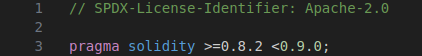
\includegraphics[width=\linewidth, keepaspectratio]{images/code_license_solidity_v.png}
        Εικόνα 1: Ορισμός άδειας και έκδοσης του Compiler της Solidity.
    \end{center}    
    
    \subsection{Structure ψηφοφορίας}
        Η δομή της ψηφοφορίας ορίζεται με τη χρήση \textbf{struct} (βλέπε Εικόνα 2) με τις ακόλουθες μεταβλητές κατάστασης (state variables):
    \begin{itemize}
        \item \textbf{string question}: για την αποθήκευση του ερωτήματος της εκάστοτε ψηφοφορίας. Είναι σημαντικό να γνωρίζουμε σε αυτό το σημείο πως μια ψηφοφορία μπορεί να απαντηθεί μόνο με ναι ή όχι.
        \item \textbf{bool isClosed}: ορίζει την κατάσταση της ψηφοφορίας, για το αν αυτή είναι ανοιχτή ή κλειστή.
        \item \textbf{mapping(address => bool) hasVoted}: για την αποθήκευση των διευθύνσεων που έχουν ψηφίσει. Το κλειδί (key) του map είναι τύπου διεύθυνσης (address) και η τιμή (value) τύπου boolean.
        \item \textbf{uint yesVotes}: για την αποθήκευση του πλήθους των θετικών ψήφων.
        \item \textbf{uint noVotes}: για την αποθήκευση του πλήθους των αρνητικών ψήφων.
    \end{itemize}
    
    \begin{center}
        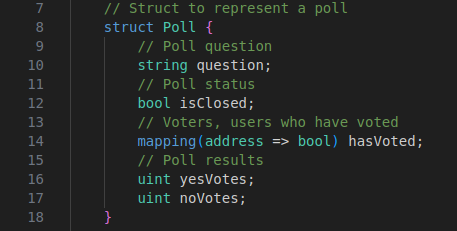
\includegraphics[width=\linewidth]{images/code_struct_poll.png}
        Εικόνα 2: Struct της ψηφοφορίας.
    \end{center}
    
    \vspace{5mm}
        Για την αποθήκευση των ψηφοφοριών που δημιουργούνται χρησιμοποιείτε μια μεταβλητή κατάστασης (state variable) με τη μορφή πίνακα (array) όπου θα περιέχει τιμές τύπου του \textbf{struct Poll}, όπως φαίνεται και στην Εικόνα 3.

    \begin{center}
        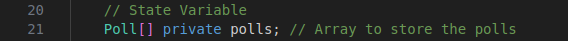
\includegraphics[width=\linewidth]{images/code_poll_state.png}
        Εικόνα 3: Array αποθήκευσης ψηφοφοριών.
    \end{center}
    
    \subsection{Function δημιουργίας νέας ψηφοφορίας}
        Για τη δημιουργία μιας νέας ψηφοφορίας χρησιμοποιείται η συνάρτηση \textbf{createNewPoll}. Αυτή η συνάρτηση δέχεται ως όρισμα την ερώτηση της νέας ψηφοφορίας από τον χρήστη. Συγκεκριμένα, η συνάρτηση δημιουργεί την ψηφοφορία και την αποθηκεύει στον πίνακα \textbf{polls}. Στη συνέχεια, αρχικοποιεί τις μεταβλητές που περιέχουν τα ακόλουθα:
        \begin{itemize}
            \item \textbf{question}: Το ερώτημα της ψηφοφορίας που δίνεται ως όρισμα από τον χρήστη.
            \item \textbf{isClosed}: Η αρχική κατάσταση της ψηφοφορίας, η οποία είναι ανοιχτή.
            \item \textbf{yesVotes}: Το αρχικό πλήθος των θετικών ψήφων, που αρχικά είναι μηδενικό.
            \item \textbf{noVotes}: Το αρχικό πλήθος των αρνητικών ψήφων, που επίσης αρχικά είναι μηδενικό.
        \end{itemize}
    
    \begin{center}
        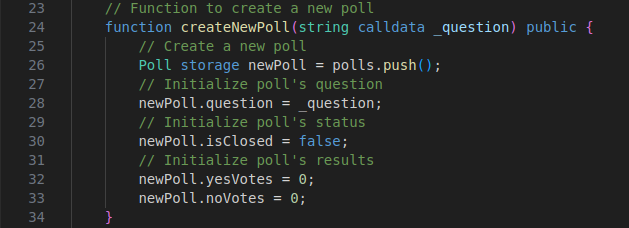
\includegraphics[width=\linewidth, keepaspectratio]{images/code_create_new_poll.png}
        Εικόνα 4: Δημιουργία μίας νέας φηφοφορίας.
    \end{center}
    
    \subsection{Function δημιουργίας ψήφου ψηφοφορίας}
        Για τη δημιουργία μιας ψήφου σε μια ψηφοφορία χρησιμοποιείται η συνάρτηση \textbf{castVote}, η οποία δέχεται ως όρισμα τον δείκτη (index) της ψηφοφορίας. Αρχικά, με τη χρήση της εντολής \textbf{require}, ελέγχεται εάν ο δείκτης της ψηφοφορίας αυτής υπάρχει στον πίνακα \textbf{polls}. Στη συνέχεια, η ψηφοφορία αυτή αποθηκεύεται προσωρινά σε μια μεταβλητή τύπου \textbf{storage}. Σε αυτό το σημείο γίνεται έλεγχος για την κατάσταση της ψηφοφορίας, εάν είναι ανοιχτή ή κλειστή, και ελέγχεται επίσης εάν ο χρήστης έχει ήδη ψηφίσει σε αυτήν. Για την απόκτηση της διεύθυνσης του χρήστη χρησιμοποιείται το αντικείμενο \textbf{msg}, το οποίο περιέχει πληροφορίες σχετικά με τη συναλλαγή. Είναι σημαντικό να σημειωθεί ότι για να αποθηκευτεί μια ψήφος στο blockchain, πρέπει να πληρούνται όλοι οι παραπάνω έλεγχοι. Εάν πληρούνται, η εκτέλεση του κώδικα του έξυπνου συμβολαίου συνεχίζεται με την καταχώρηση της ψήφου, αυξάνοντας την αντίστοιχη μεταβλητή είτε για τις θετικές είτε για τις αρνητικές ψήφους.

        
    \begin{center}
        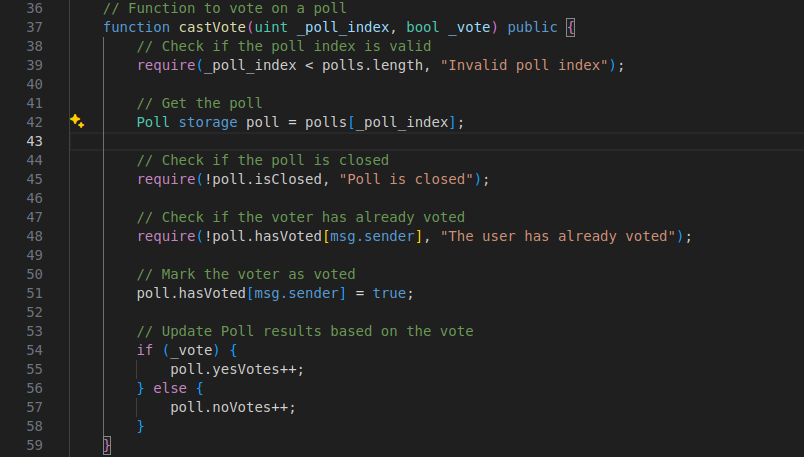
\includegraphics[width=\linewidth, keepaspectratio]{images/code_cast_vote.png}
        Εικόνα 5: Δημιουργία ψήφου.
    \end{center}
    
    \subsection{Function κλείσιμο ψηφοφορίας}
        Για το κλείσιμο μιας ψηφοφορίας χρησιμοποιείται η συνάρτηση \textbf{"closePoll"} η οποία δέχεται ως όρισμα τον δείκτη (index) της ψηφοφορίας. Αρχικά με την χρήση μιας εντολής \textbf{require} ελέγχει εάν ο δείκτης της συγκεκριμένης ψηφοφορίας υπάρχει στον πίνακα \textbf{"polls"}. Στην συνέχεια βρίσκει και αποθηκεύει προσωρινά σε μια μεταβλητή τύπου \textbf{storage} την ψηφοφορία αυτή και στο σημείο αυτό ελέγει την κατάσταση της ψηφοφορίας αν είναι ήδη κλειστή. Στην περίπτωση που τηρούνται τα παραπάνω αλλάζει η κατάσταση (status) της ψηφοφορίας σε "κλειστή" μεταβάλοντας την τιμή στην μεταβλητή κατάστασης (state variable) \textbf{"isClosed"}.
    
    \begin{center}
        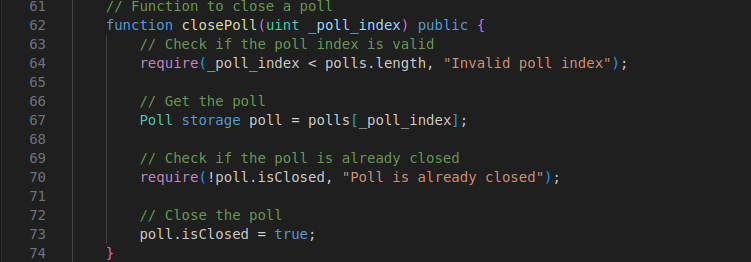
\includegraphics[width=\linewidth, keepaspectratio]{images/code_close_poll.png}
        Εικόνα 6: Κλείσιμο μίας ψηφοφορίας.
    \end{center}
    
    \subsection{Function προβολή αποτελεσμάτων ψηφοφορίας}
        Για την προβολή των αποτελεσμάτων μιας ψηφοφορίας χρησιμοποιείται η συνάρτηση \textbf{"showPollResults"} η οποία δέχεται ως όρισμα τον δείκτη (index) της ψηφοφορίας. Αρχικά με την χρήση μιας εντολής \textbf{require} ελέγχει εάν ο δείκτης της συγκεκριμένης ψηφοφορίας υπάρχει στον πίνακα \textbf{"polls"}. Στην περίπτωση που τηρείται η παραπάνω συνθήκη βρίσκει και αποθηκεύει προσωρινά σε μια μεταβλητή τύπου \textbf{storage} την ψηφοφορία αυτή. Τέλος, η συνάρτηση επιστρέφει με δύο ακέραιους αριθμούς το πλήθος των θετικών \textbf{"yesVotes"} και αρνητικών \textbf{"noVotes"} ψήφων.

    \begin{center}
        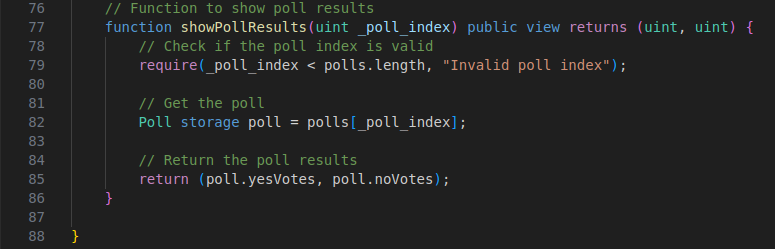
\includegraphics[width=\linewidth, keepaspectratio]{images/code_show_poll_results.png}
        Εικόνα 7: Εμφάνιση αποτελεσμάτων μίας ψηφοφορίας.
    \end{center}
    
    \newpage
    
\section{Παράδειγμα Εκτέλεσης}

    Για την εκτέλεση του συμβολαίου χρησιμοποιήθηκε το \textbf{Remix IDE} λόγω φιλικού χρηστικού περιβάλλοντος.
    
    \subsection{Δημιουργία Νέας Ψηφοφορίας}
    
    \begin{center}
        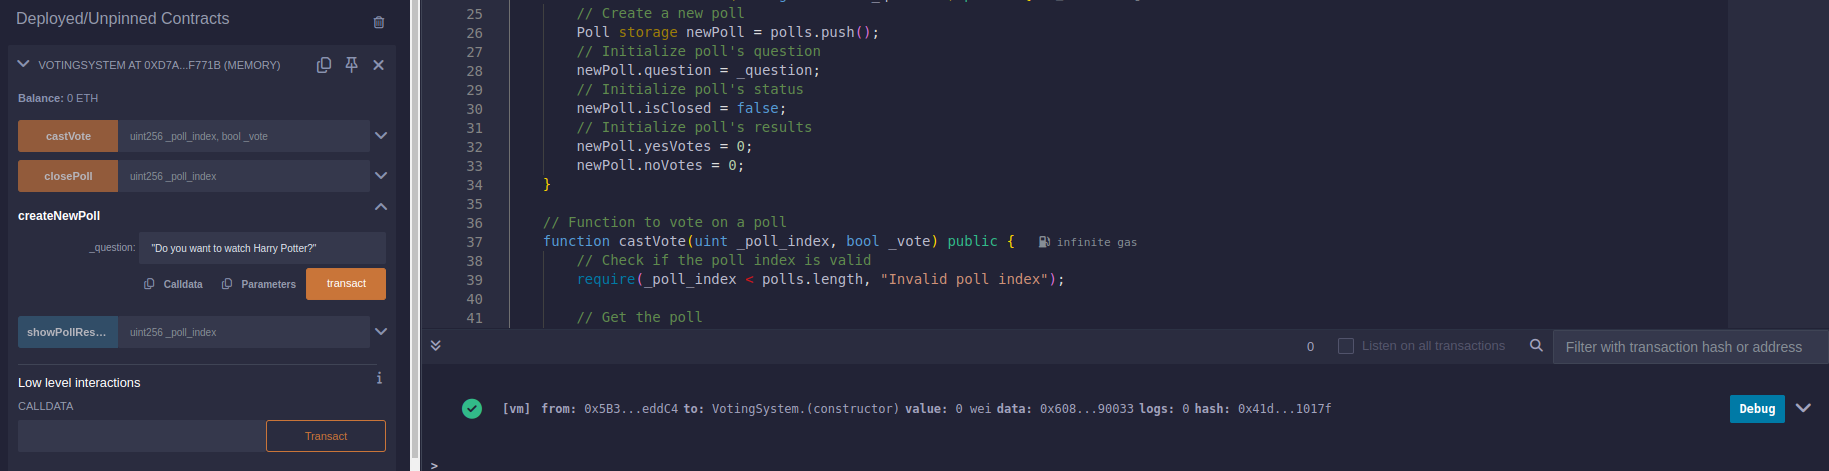
\includegraphics[width=\linewidth, keepaspectratio]{images/ss_create_new_poll.png}
        Εικόνα 8: Δημιουργία μίας ψηφοφορίας.
    \end{center}
    
    \subsection{Ψήφος σε Ψηφοφορία}
    
    \begin{center}
        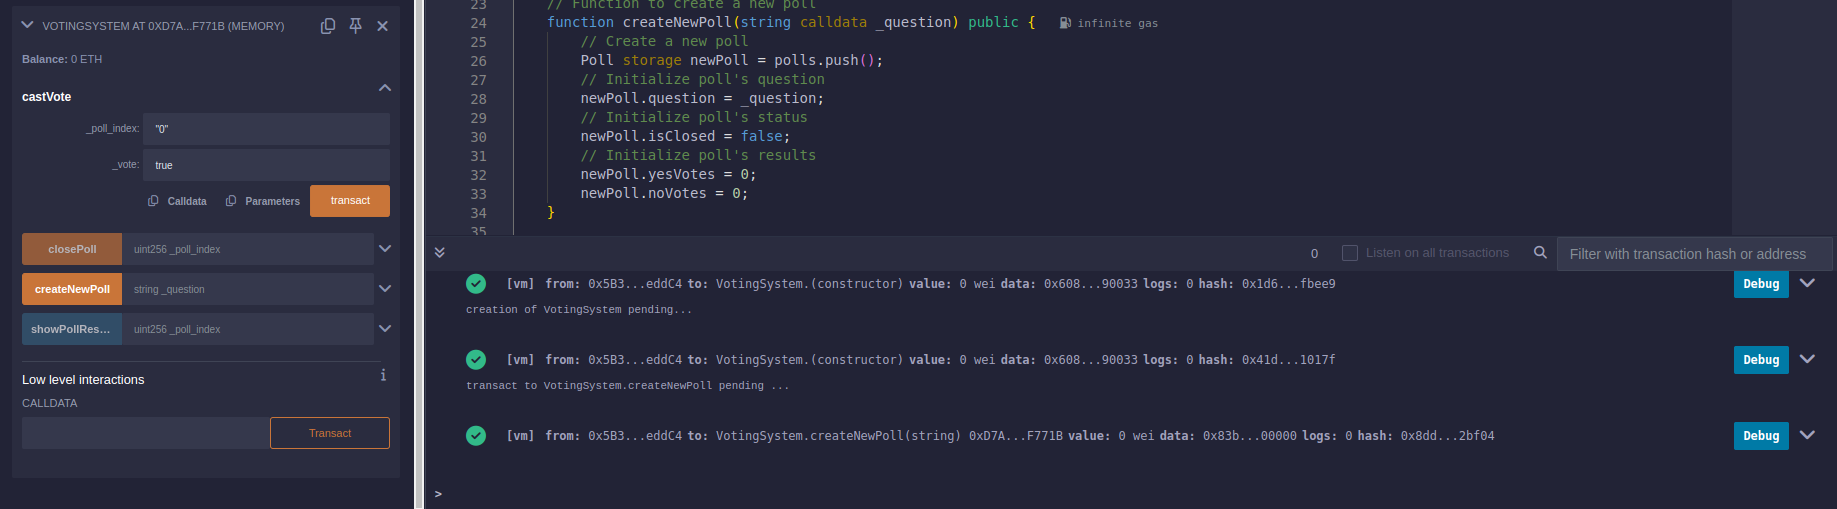
\includegraphics[width=\linewidth, keepaspectratio]{images/ss_cast_vote.png}
        Εικόνα 9: Δημιουργία Ψήφου.
    \end{center}
    
    \begin{center}
        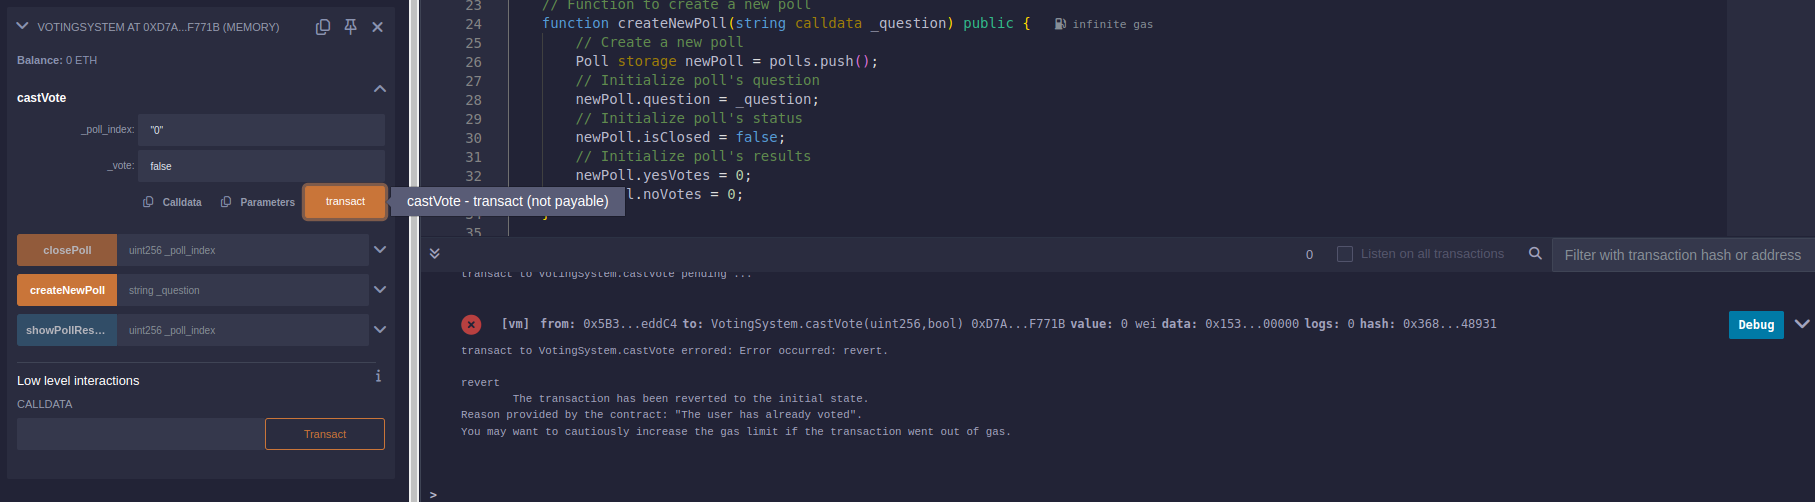
\includegraphics[width=\linewidth, keepaspectratio]{images/ss_cast_vote_denied.png}
        Εικόνα 10: Άρνηση αποδοχής ψήφου από χρήστη που έχει ήδη ψηφίσει.
    \end{center}
    
    \subsection{Κλείσιμο Ψηφοφορίας}
    
    \begin{center}
        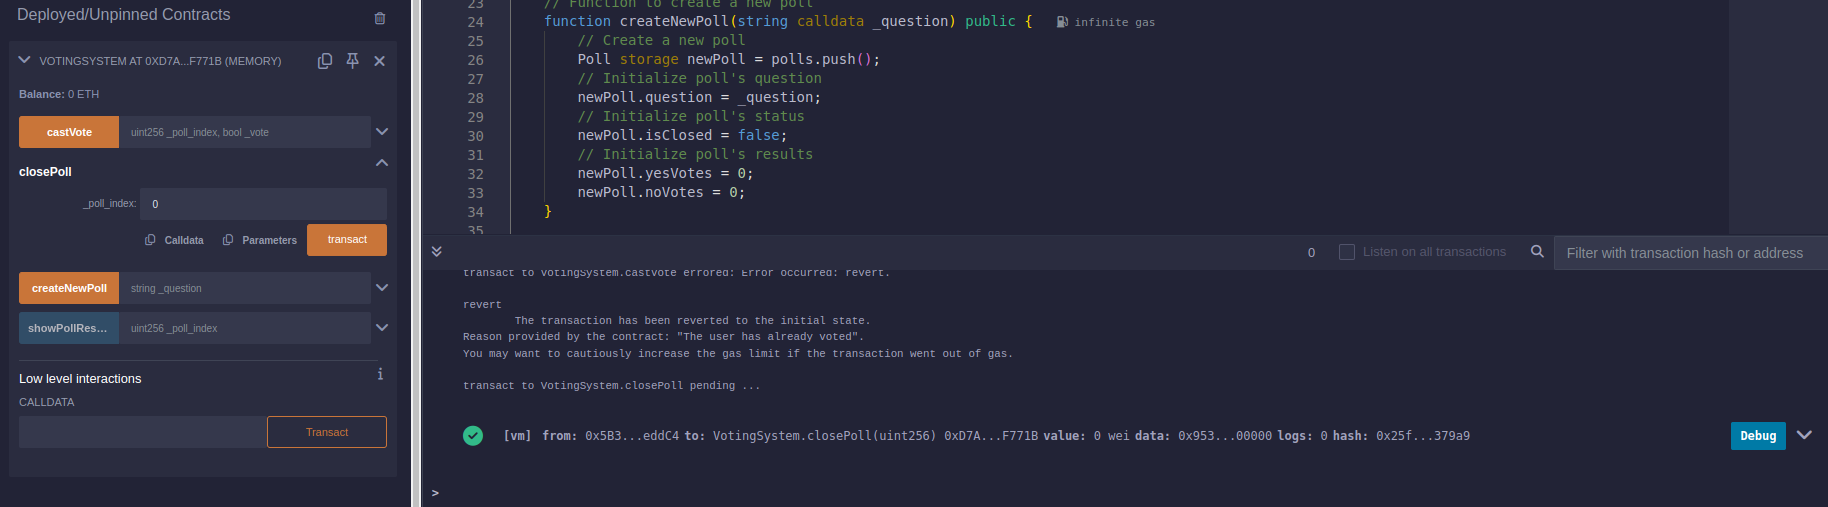
\includegraphics[width=\linewidth, keepaspectratio]{images/ss_close_vote.png}
        Εικόνα 11: Κλείσιμο Ψηφοφορίας.
    \end{center}
    
    \subsection{Προβολή Αποτελεσμάτων}
    
    \begin{center}
        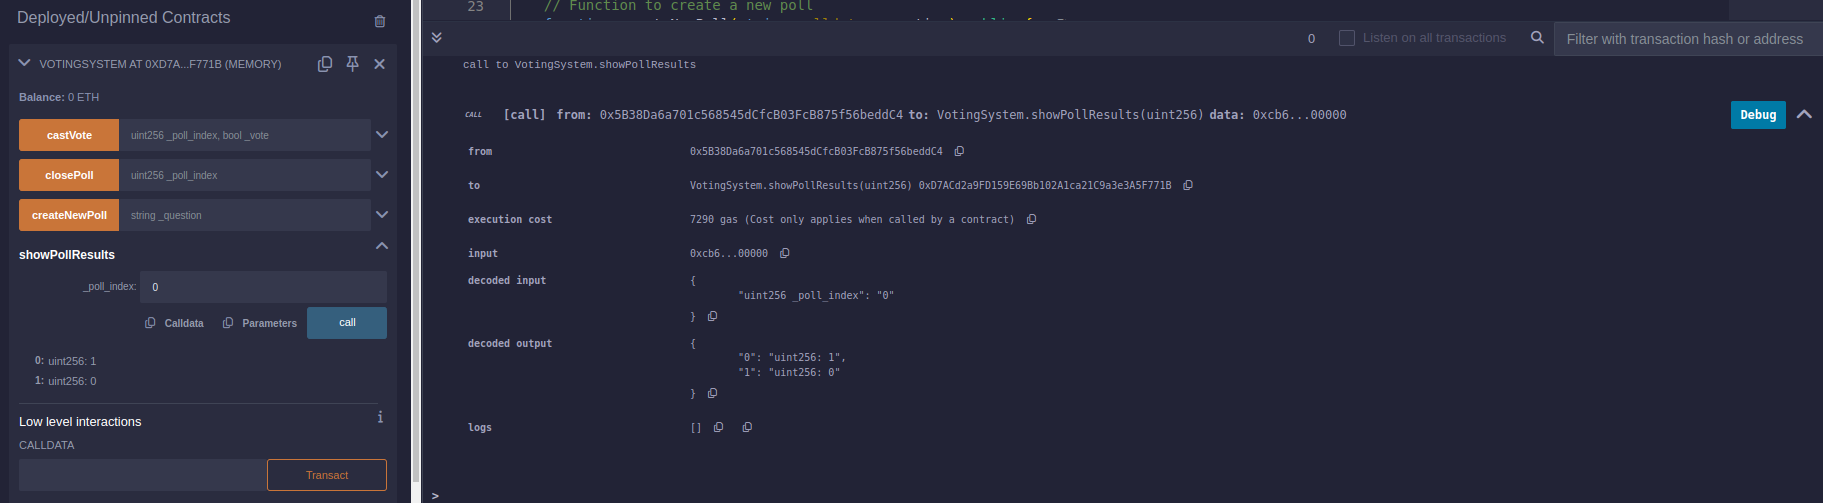
\includegraphics[width=\linewidth, keepaspectratio]{images/ss_show_poll_results.png}
        Εικόνα 12: Εμφάνιση Αποτελεσμάτων Ψηφοφορίας.
    \end{center}

\newpage

\section{Πηγές}

\begin{enumerate}
    \item \textbf{Παρουσίαση Solidity:} \\
    \textit{Εισαγωγή στη Solidity} \\
    Available online: \url{https://thales.cs.unipi.gr/modules/document/file.php/TMD140/%CE%94%CE%B9%CE%B1%CE%BB%CE%AD%CE%BE%CE%B5%CE%B9%CF%82%20%CE%9C%CE%B1%CE%B8%CE%AE%CE%BC%CE%B1%CF%84%CE%BF%CF%82%202024/solidity.pdf} \\
    Accessed on: 11/07/2024
    
    \item \textbf{Παρουσίαση Solidity:} \\
    \textit{Remix Μεταβλητές κατάστασης \& ορατότητα} \\
    Available online: \url{https://thales.cs.unipi.gr/modules/document/file.php/TMD140/%CE%94%CE%B9%CE%B1%CE%BB%CE%AD%CE%BE%CE%B5%CE%B9%CF%82%20%CE%9C%CE%B1%CE%B8%CE%AE%CE%BC%CE%B1%CF%84%CE%BF%CF%82%202024/solidity_2.pdf} \\
    Accessed on: 11/07/2024
\end{enumerate}

\end{document}